\section{Implementation}
\label{sec:impl}
We have implemented a monitoring system for Node.js consisting of two main components, as depicted in \Cref{fig:arch}.

\begin{figure}
\centering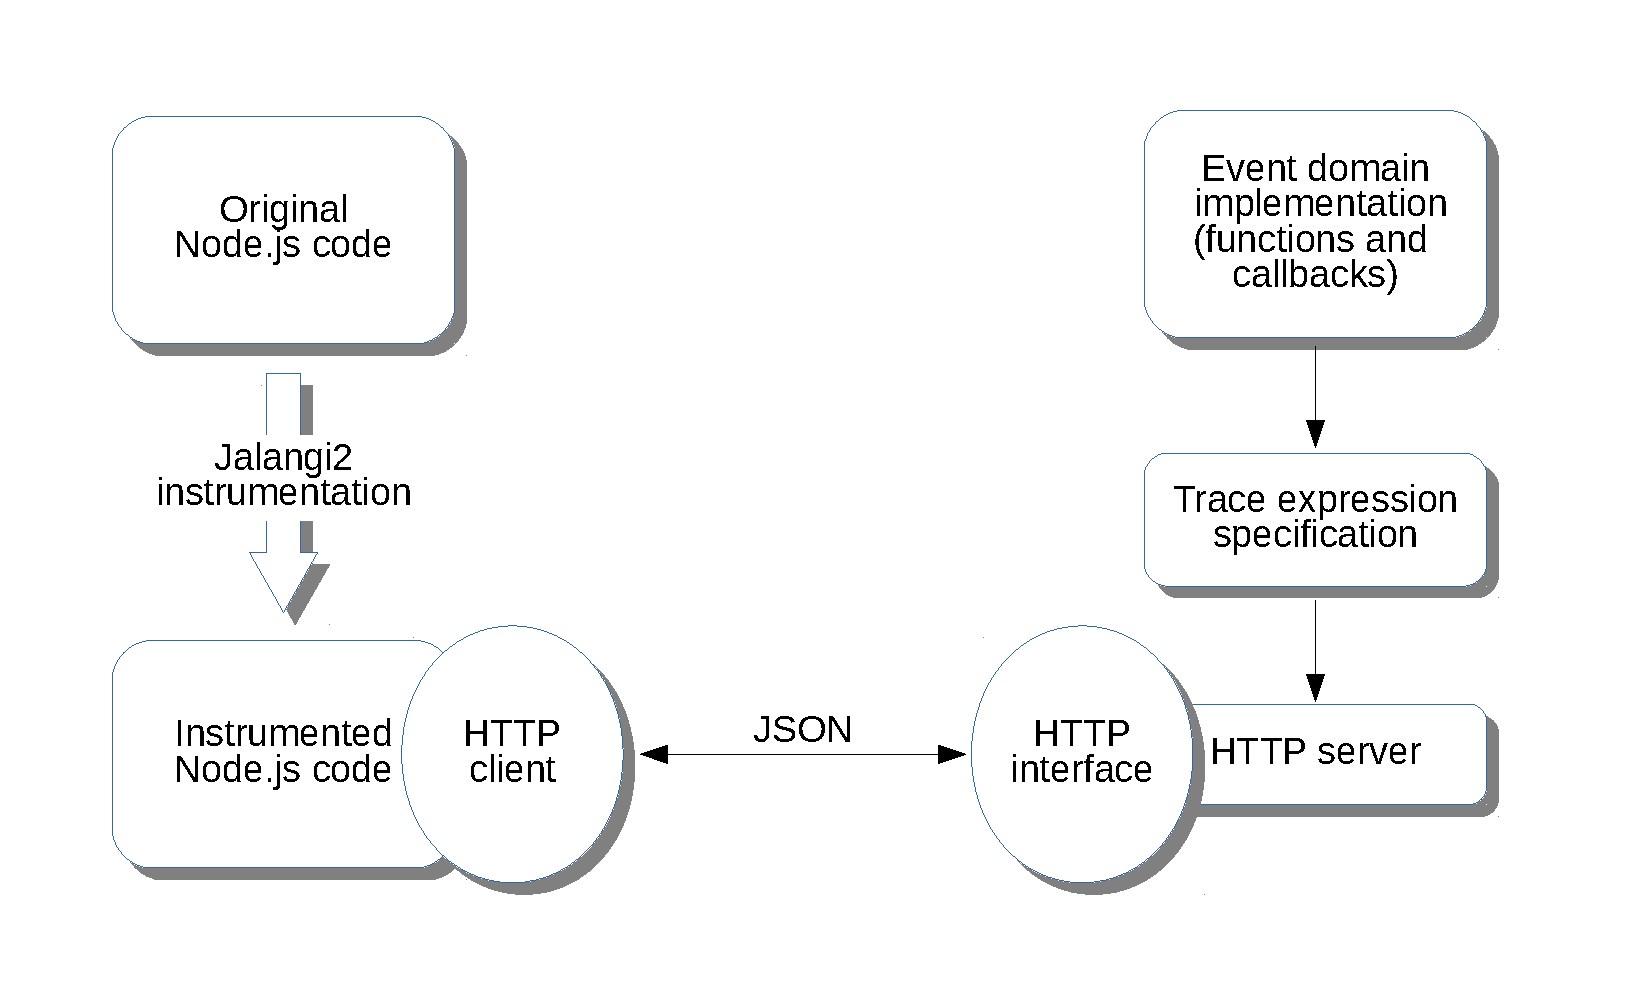
\includegraphics[width=.8\textwidth]{fig/architecture}
\caption{Monitoring architecture for Node.js exploiting SWI-Prolog server with an HTTP interface.}
\label{fig:arch}
\end{figure}

The component on the left-hand-side has been developed in JavaScript and is responsible for emitting through \emph{code instrumentation} all relevant events that have to be monitored
at runtime, while the other on the right-hand-side consists of an HTTP server, written in SWI-Prolog, which receives from the instrumented code all monitored events in form of HTTP requests in JSON format, and checks them against a specification consisting of Prolog components defining the used event domain and trace expression; in case the server detects an error because the received event does not meet the specification, it sends back details about the failure in response to the client. Implementation through an HTTP server allows decoupling of the monitored system from the monitor, and
favor interoperability, and runtime verification of distributed systems.

%% Further details on the approach and the implementation with Jalangi2 can be found in the related paper \cite{TowardsIoT17}.

%% The core idea is to modify the original source code of the program to be monitored in a way that allows observation of relevant events.
%% Once an event is observed, the monitor can verify it against the specification, eventually acting in case of erroneous behavior.

\subsection*{Instrumentation}
We have employed \emph{Jalangi2} \cite{jalangi}, a mature tool supporting instrumentation with 
% gia' linkato nelle prime pagine
%\footnote{\url{https://github.com/Samsung/jalangi2}} \cite{jalangi}
arbitrary code which can be inserted right before or after any main JavaScript operation: access to properties, declarations, functions and methods invocation, among others. Jalangi2 also gives access to information about the operation itself, as the arguments of a function call or the target object of a property access.
The tool allows for state-of-the-art performance in the context of code instrumentation for dynamic analysis.
To the best of our knowledge, the most similar tool is Linvail \cite{linvail}, though its performance are reported to be worst by an order of magnitude (w.r.t.\ the overhead).

Despite the flexibility of Jalangi2, instrumenting code to determine when asynchronous calls and their callbacks are executed and to send the corresponding events in form of an HTTP request was a challenging task, that required to develop more than 450 SLOC of non trivial JavaScript code, to tackle
several issues, among which the following ones are the most significant:

\begin{itemize}
\item Anonymous and arrow functions are extremely common in JavaScript and Node.js applications, and the information about their name
  provided by Jalangi2 for function calls is completely  useless, hence we had to implement from scratch a reliable mechanism to identify them.
\item Jalangi2 does not provide any mechanism for coupling asynchronous function calls with their callbacks, a feature which is
  necessary to allow RV to detect undesired non-deterministic behavior due to the invalid use of asynchronous operations, as shown in
  \Cref{sec:examples}. %% the same asynchronous function can be used multiple times with different arguments and callbacks, and vice versa.
To this aim, the instrumentation we have implemented dynamically wraps callbacks \emph{at runtime} and generate a unique identifier for each one of them.
\item Jalangi2 allows insertion of instrumented code for function calls at four different sites: before and after a function call (caller sites), 
  before the execution of a function body starts, and after the execution of a function body completes (callee sites). Since
  events are tracked through code instrumentation, all four kinds of sites are useful for library functions that cannot be
  instrumented (either because they are not implemented in JavaScript, or because instrumentation would imply a severe performance penalty):  the caller sites
  are used when calls to library functions have to be monitored, while the callee sites are useful to track calls to callbacks that are passed to
  library functions.

  This flexibility comes at a cost when monitoring functions whose source code is available because they are part of the very same program under analysis; in this case two duplicate events would be generated as HTTP client requests sent to the monitoring Prolog server. To this aim,
  the instrumentation we have implemented keeps track of all kinds of function calls, to avoid such duplications.
  
\item In case of method calls, it is useful to identify the target object on which the method has been called, to keep track of the correct
  flow of methods that can be safely invoked on a specific object; Jalangi2 solves this problem only partially,
  because it exposes  the target objects of method calls as mere JavaScript values, without information on the identity of the objects.
  Since the information carried by events are converted into JSON format before sending them to the monitoring server, the identity of objects are lost 
  in such a conversion. Our implementation uses a weak map to keep track of object identities and to generate events containing a unique identifier
  for target objects of method calls; a weak map is employed to avoid issues with garbage collection.

\item Though JSON is a natural fit for JavaScript objects serialization, some important aspects needed to be handled.
Objects containing circular references, for instance, are quite common in Node.js modules, but they cannot be encoded in JSON, and the JavaScript standard library serialization (\lstinline|JSON.stringify|) throws an error on such objects.
Furthermore, JavaScript supports getters, which are special functions invoked when a property is accessed.
During experiments with the \lstinline{http} module, we found that some modules add getter functions to objects before their code can actually be
correctly executed; unfortunately, the standard serialization offered by \lstinline|JSON.stringify| invokes getters during stringification, hence
JSON conversion  breaks if an object contains a getter performing some illegal operation. 
For these reasons, we have  adapted the JSON serialization process by providing a suitable replacer\footnote{See the code at \url{https://github.com/LucaFranceschini/trace-expressions/blob/master/jalangi/stringify-trunc.js}} able to correctly deal
with cyclic objects and getters.

\end{itemize}
Note that even if we strongly rely on Jalangi2, these issues need to be faced with any code instrumentation framework when applied to Node.js code, because of the very nature of the framework and of JavaScript itself.

Our prototype implementation enriches the capabilities of Jalangi by supporting these additional features for Node.js monitoring.
We are currently looking at proxy-based alternative approaches based on reflection rather than instrumentation, since proxies \cite{proxy} are now natively supported by JavaScript.

The current implementation of trace expression semantics is coded in SWI-Prolog, since logic programming is a natural fit for inference rules and transition systems, and cyclic terms are supported by the \texttt{coinduction} library \cite{CoLP06}.


Another challenge consisted in avoiding the performance penalties we detected with the first version of the
instrumenting code: the file explorer server employed in our benchmarks (see Section~\ref{sec:exps}) could serve no more than
three requests per second when monitored; that was an unacceptable result even when limiting
the use of runtime verification to the development stage for debugging and testing purposes.

A first practical way to obtain a speed up of the monitored application consisted in
avoiding the monitored application to directly synchronize with the monitoring Prolog server;
synchronous communication guarantees that the monitor always receives events in the correct order,
but has a negative effect on performances. To avoid this problem, we let the instrumented code
to asynchronously interact with a child process by sending to it all relevant events. Synchronous
communication with the Prolog  monitor is managed by the child process.

Another useful optimization consisted in reducing the network traffic 
between the monitored application and the monitor; while
the first version of the instrumentation was designed to send
all detected events, the optimization version sends only those events 
which are relevant for the verification.

%% This work is a preliminary step towards runtime verification of Internet of Things applications,
%% both because Node.js is emerging as a standard framework for IoT development, and the implementation through an HTTP
%% server offers a natural support to verification of distributed systems, where (instrumented) devices can send events to a monitoring server.

